% Options for packages loaded elsewhere
\PassOptionsToPackage{unicode}{hyperref}
\PassOptionsToPackage{hyphens}{url}
\PassOptionsToPackage{dvipsnames,svgnames*,x11names*}{xcolor}
%
\documentclass[
]{article}
\usepackage{lmodern}
\usepackage{amsmath}
\usepackage{ifxetex,ifluatex}
\ifnum 0\ifxetex 1\fi\ifluatex 1\fi=0 % if pdftex
  \usepackage[T1]{fontenc}
  \usepackage[utf8]{inputenc}
  \usepackage{textcomp} % provide euro and other symbols
  \usepackage{amssymb}
\else % if luatex or xetex
  \usepackage{unicode-math}
  \defaultfontfeatures{Scale=MatchLowercase}
  \defaultfontfeatures[\rmfamily]{Ligatures=TeX,Scale=1}
\fi
% Use upquote if available, for straight quotes in verbatim environments
\IfFileExists{upquote.sty}{\usepackage{upquote}}{}
\IfFileExists{microtype.sty}{% use microtype if available
  \usepackage[]{microtype}
  \UseMicrotypeSet[protrusion]{basicmath} % disable protrusion for tt fonts
}{}
\makeatletter
\@ifundefined{KOMAClassName}{% if non-KOMA class
  \IfFileExists{parskip.sty}{%
    \usepackage{parskip}
  }{% else
    \setlength{\parindent}{0pt}
    \setlength{\parskip}{6pt plus 2pt minus 1pt}}
}{% if KOMA class
  \KOMAoptions{parskip=half}}
\makeatother
\usepackage{xcolor}
\IfFileExists{xurl.sty}{\usepackage{xurl}}{} % add URL line breaks if available
\IfFileExists{bookmark.sty}{\usepackage{bookmark}}{\usepackage{hyperref}}
\hypersetup{
  pdftitle={MSDS 7333 Spring 2021: Case Study 02},
  pdfauthor={Sachin Chavan,Tazeb Abera,Gautam Kapila,Sandesh Ojha},
  colorlinks=true,
  linkcolor=Maroon,
  filecolor=Maroon,
  citecolor=Blue,
  urlcolor=gray,
  pdfcreator={LaTeX via pandoc}}
\urlstyle{same} % disable monospaced font for URLs
\usepackage[margin=1in]{geometry}
\usepackage{color}
\usepackage{fancyvrb}
\newcommand{\VerbBar}{|}
\newcommand{\VERB}{\Verb[commandchars=\\\{\}]}
\DefineVerbatimEnvironment{Highlighting}{Verbatim}{commandchars=\\\{\}}
% Add ',fontsize=\small' for more characters per line
\usepackage{framed}
\definecolor{shadecolor}{RGB}{248,248,248}
\newenvironment{Shaded}{\begin{snugshade}}{\end{snugshade}}
\newcommand{\AlertTok}[1]{\textcolor[rgb]{0.94,0.16,0.16}{#1}}
\newcommand{\AnnotationTok}[1]{\textcolor[rgb]{0.56,0.35,0.01}{\textbf{\textit{#1}}}}
\newcommand{\AttributeTok}[1]{\textcolor[rgb]{0.77,0.63,0.00}{#1}}
\newcommand{\BaseNTok}[1]{\textcolor[rgb]{0.00,0.00,0.81}{#1}}
\newcommand{\BuiltInTok}[1]{#1}
\newcommand{\CharTok}[1]{\textcolor[rgb]{0.31,0.60,0.02}{#1}}
\newcommand{\CommentTok}[1]{\textcolor[rgb]{0.56,0.35,0.01}{\textit{#1}}}
\newcommand{\CommentVarTok}[1]{\textcolor[rgb]{0.56,0.35,0.01}{\textbf{\textit{#1}}}}
\newcommand{\ConstantTok}[1]{\textcolor[rgb]{0.00,0.00,0.00}{#1}}
\newcommand{\ControlFlowTok}[1]{\textcolor[rgb]{0.13,0.29,0.53}{\textbf{#1}}}
\newcommand{\DataTypeTok}[1]{\textcolor[rgb]{0.13,0.29,0.53}{#1}}
\newcommand{\DecValTok}[1]{\textcolor[rgb]{0.00,0.00,0.81}{#1}}
\newcommand{\DocumentationTok}[1]{\textcolor[rgb]{0.56,0.35,0.01}{\textbf{\textit{#1}}}}
\newcommand{\ErrorTok}[1]{\textcolor[rgb]{0.64,0.00,0.00}{\textbf{#1}}}
\newcommand{\ExtensionTok}[1]{#1}
\newcommand{\FloatTok}[1]{\textcolor[rgb]{0.00,0.00,0.81}{#1}}
\newcommand{\FunctionTok}[1]{\textcolor[rgb]{0.00,0.00,0.00}{#1}}
\newcommand{\ImportTok}[1]{#1}
\newcommand{\InformationTok}[1]{\textcolor[rgb]{0.56,0.35,0.01}{\textbf{\textit{#1}}}}
\newcommand{\KeywordTok}[1]{\textcolor[rgb]{0.13,0.29,0.53}{\textbf{#1}}}
\newcommand{\NormalTok}[1]{#1}
\newcommand{\OperatorTok}[1]{\textcolor[rgb]{0.81,0.36,0.00}{\textbf{#1}}}
\newcommand{\OtherTok}[1]{\textcolor[rgb]{0.56,0.35,0.01}{#1}}
\newcommand{\PreprocessorTok}[1]{\textcolor[rgb]{0.56,0.35,0.01}{\textit{#1}}}
\newcommand{\RegionMarkerTok}[1]{#1}
\newcommand{\SpecialCharTok}[1]{\textcolor[rgb]{0.00,0.00,0.00}{#1}}
\newcommand{\SpecialStringTok}[1]{\textcolor[rgb]{0.31,0.60,0.02}{#1}}
\newcommand{\StringTok}[1]{\textcolor[rgb]{0.31,0.60,0.02}{#1}}
\newcommand{\VariableTok}[1]{\textcolor[rgb]{0.00,0.00,0.00}{#1}}
\newcommand{\VerbatimStringTok}[1]{\textcolor[rgb]{0.31,0.60,0.02}{#1}}
\newcommand{\WarningTok}[1]{\textcolor[rgb]{0.56,0.35,0.01}{\textbf{\textit{#1}}}}
\usepackage{longtable,booktabs}
\usepackage{calc} % for calculating minipage widths
% Correct order of tables after \paragraph or \subparagraph
\usepackage{etoolbox}
\makeatletter
\patchcmd\longtable{\par}{\if@noskipsec\mbox{}\fi\par}{}{}
\makeatother
% Allow footnotes in longtable head/foot
\IfFileExists{footnotehyper.sty}{\usepackage{footnotehyper}}{\usepackage{footnote}}
\makesavenoteenv{longtable}
\usepackage{graphicx}
\makeatletter
\def\maxwidth{\ifdim\Gin@nat@width>\linewidth\linewidth\else\Gin@nat@width\fi}
\def\maxheight{\ifdim\Gin@nat@height>\textheight\textheight\else\Gin@nat@height\fi}
\makeatother
% Scale images if necessary, so that they will not overflow the page
% margins by default, and it is still possible to overwrite the defaults
% using explicit options in \includegraphics[width, height, ...]{}
\setkeys{Gin}{width=\maxwidth,height=\maxheight,keepaspectratio}
% Set default figure placement to htbp
\makeatletter
\def\fps@figure{htbp}
\makeatother
\setlength{\emergencystretch}{3em} % prevent overfull lines
\providecommand{\tightlist}{%
  \setlength{\itemsep}{0pt}\setlength{\parskip}{0pt}}
\setcounter{secnumdepth}{-\maxdimen} % remove section numbering
\usepackage{fancyhdr}
\pagestyle{fancy}
\fancyhead[L]{Case Study 02}
\usepackage{float}
\ifluatex
  \usepackage{selnolig}  % disable illegal ligatures
\fi

\title{MSDS 7333 Spring 2021: Case Study 02}
\usepackage{etoolbox}
\makeatletter
\providecommand{\subtitle}[1]{% add subtitle to \maketitle
  \apptocmd{\@title}{\par {\large #1 \par}}{}{}
}
\makeatother
\subtitle{Analysis of Runners' Performance}
\author{Sachin Chavan,Tazeb Abera,Gautam Kapila,Sandesh Ojha}
\date{2021 February 01}

\begin{document}
\maketitle

\hypertarget{introduction}{%
\section{Introduction}\label{introduction}}

This is an information age and there is lot of data generated and
published every day in different forms. If we just think about websites
there are hundreds of thousands of websites across the world publish
different types of content like research, news, education,blogs etc
everyday and most of it is freely available to read and digest. Such
information can be potentially be useful in gaining insights for
personal and professional interests. e.g.~we can learn lot about
population like education, labor, gender distribution etc with exploring
data from the census data published on world bank or census.gov. This is
all available for free to download and view on such websites.

In this case study we are going to explore one of such website
\href{http://www.cherryblossom.org/}{www.cherryblossom.org}.
\textbf{Cherry blossom Ten Mile Run} is annual 10-mile road race in
Washington, D.C. founded in 1973, almost 48 years ago and its popularity
and participation in the event has grown over the years. As per their
website in year 2018 around 17000 people participated in the race
ranging in age 9 to 89 years. Textbook has covered Male racers in its
example, we are going to explore Female racers. We will study how age
affect physical performance in female racers and try to get many other
insights hidden in the data.

\emph{``According to Bureau for labor Statistics, road running is third
most common form of sport and exercise activity among Americans.''}
{[}2{]}

\hypertarget{business-understanding}{%
\section{Business Understanding}\label{business-understanding}}

The purpose of the case study is to gather meaningful insights from
women participant's results that are published on famous Cherry Blossom'
website for the years 1999-2012 under 10 mile race category. The primary
objective is to download the 1999 to 2012 results of 10 mile running
event from the website to explore and shed light on the effect of age on
the runner's physical performance over the years along with other
meaningful insights if any.

The Cherry Blossom organizes 5K and 10M running event year in
Washington,D.C early in April when cherry trees are said to be in bloom.
They record results for every participants and publish on their website.
The race has been in such demand that the runner are chosen via lottery
system to enter the race. Participants have different age range and for
both male and female, however, this case study focuses on Woman's
result.

\hypertarget{objective}{%
\subsection{Objective}\label{objective}}

Download the woman's results for the duration of 1999-2012 from Cherry
Blossom's website, perform data wrangling and gather meaningful
insights.

\newpage

\hypertarget{data-extraction-preparation}{%
\section{Data Extraction /
Preparation}\label{data-extraction-preparation}}

At the time of writing this document
\href{http://www.cherryblossom.org/}{www.cherryblossom.org} was revamped
and they have made results available in tabular format on
\href{http://www.cballtimeresults.org/performances}{http://www.cballtimeresults.org}.
Based on new web page that they have designed it can list results based
on option selected in the dropdowns and all results are paginated with
one page shows 20 results. So result for selected year is spanned across
multiple pages for selected year of result. There is no way data can be
extracting manually. This has to be automated by method called Web
scraping. The program will automatically scrape through pages and
extract records for our analysis.

The new Cherry blossom results pages are not dynamic content and it
makes somewhat easier to pull all required records from the website.

e.g URL for First page of 1999 Woman's results for 10 Mile run:

\url{http://www.cballtimeresults.org/performances?division=Overall+Women\&page=1\&section=10M\&sex=W\&utf8=\&year=1999}

\begin{figure}[H]

{\centering 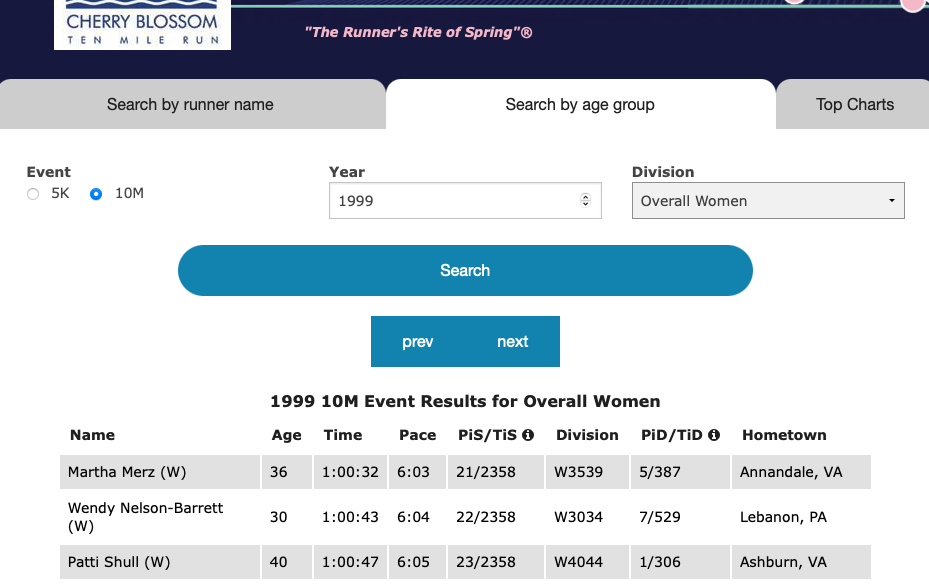
\includegraphics[width=1\linewidth,height=1\textheight,]{images/results_page} 

}

\caption{Results Page}\label{fig:unnamed-chunk-3}
\end{figure}

URL pattern was observed same for all pages, records for all runners for
selected years can be extracted just by changing values of

\begin{itemize}
\tightlist
\item
  Page Number - \emph{{[}page= {]}}
\item
  Race Year - \emph{{[}year= {]}}
\end{itemize}

Following attributes remains same for our purpose as case study is
limited to analysis of women racers.

\begin{itemize}
\tightlist
\item
  Division - \emph{{[}division=Overall+Women{]}}
\item
  Sex - \emph{{[}sex=W{]}}
\item
  section - \emph{{[}section=10M{]}}
\end{itemize}

As seen in screenshot results are presented in tabular format. So web
scraping is the method needs to be utilized to extract data from these
results pages. R programming langauge comes with sophisticated technique
to scrape through web pages to extract records from html tables. R
package \textbf{rvest} provides interfaces which can accept URL and tags
from which data to be extracted. Most of HTML parsing is done by rvest
package but it does not format data to put in R dataframe. So additional
programming is required to format data that is pulled from webpages.

So to pull data from results web pages following things are required:

\begin{itemize}
\tightlist
\item
  Use R rvest package to parse HTML page with required tags. read\_html,
  html\_nodes, html\_text are the supporting functions that will be used
  to extract tabular data.
\item
  Regular expressions are also helpful sometimes to find specic pattern
  in strings. e.g.~time column has specific format HH:MM:SS.Where HH, MM
  and SS are digits. Regular expressions are useful to check if time
  column contains data that contains other than colon and digits.
\item
  Format records returned by \textbf{rvest} functions
\item
  String manipulations are required to format data
\item
  Put data in R Data Frame and do further wrangling, once data was
  extracted.
\end{itemize}

\hypertarget{constraints}{%
\subsection{Constraints}\label{constraints}}

Web scraping comes with limitations. Programs developed to pull data
from the websites cannot be generalized much and it heavily dependent on
design of the web pages. Although, no one changes web page design that
frequently, it is required for us to check if there are any changes in
the web pages, structure of data etc to extract data from the website.
Programs are needs to be updated if there is any change in the content
on the web page. In general following things to needs to be taken into
considerations when using web scraping to extract data

\begin{itemize}
\tightlist
\item
  URL - It may change. For cherry blossom results URL has similar format
  for all results. so we just have to change few parameters in the URL
  to retrieve required result. But that may not be the case always. URL
  may need to checked and program may need to be reconfigured.
\item
  If data is in tabular format like in the case of Cherry Blossom
  website, they may add more columns or remove existing columns. So one
  has to keep checking on the structure of the data that they are
  scraping.
\item
  Dynamic contents are even more challenging. In the case of dynamic
  content and URL to access is may not be that sophisticated as we found
  in Cherry Blossom website.
\item
  Websites normally puts restrictions amount of to be extracted in
  single timeframe so large scale data extraction is harder.
\item
  Robots.txt - This is very important. This file is used to manage
  traffic to the website. One should look at this file which is
  generally located at
  \href{http://www.cherryblossom.org/robots.txt}{http://www.abc.com/robots.txt}
  to see if website allows web scraping/crawling. This is not the hard
  rule to follow what is written in the \textbf{robots.txt} but
  violation could lead to legal troubles.
\item
  The targeted website can also block web crawler's IP address
  permanently if guidelines are not followed.
\item
  R provides R package to extract data from website, but it does not
  support everything. There are many other tools available with R and
  Python that developers need to keep themselves updated instead of
  reinventing the wheel.
\end{itemize}

\newpage

\hypertarget{data-extraction-execution}{%
\section{Data Extraction / Execution}\label{data-extraction-execution}}

First step in extracting data from the website is crawl through
different web pages by changing parameters in the URL as mentioned in
previous section. Extract following fields for each runner, which in
later steps can be restrcutred the desired format.

\begin{longtable}[]{@{}ll@{}}
\caption{Data Fields on the Website}\tabularnewline
\toprule
Field Name & Field Description\tabularnewline
\midrule
\endfirsthead
\toprule
Field Name & Field Description\tabularnewline
\midrule
\endhead
Year & Year of participation\tabularnewline
Name & Last Name and First Name of the Runner\tabularnewline
Age & Age\tabularnewline
Pace & Miles per hour\tabularnewline
PiSTiS & Rank of the runner in Male/Female category\tabularnewline
Division & Division\tabularnewline
PiDTiD & Rank in Runner's Division\tabularnewline
HomeTown & Runner's Home Town\tabularnewline
\bottomrule
\end{longtable}

Data extracted from the wesbite loaded into R dataframe. R's rvest
package was used to extract data from the HTML page on the Cherry
Blossom website. All R methods are written in \emph{cs02\_methods.R}
file. Method \emph{loadDF} calls rvest functions \emph{read\_html},
\emph{html\_text}, regular expression along with custom made functions
getURL, getPlayerRecord to read player's record to store into R
dataframe. Values of the fields were loaded as it is from the HTML
tables to R dataframe. First five records are as shown in below table.

\begin{longtable}[]{@{}rlrllllll@{}}
\caption{Runner's data parsed into dataframe}\tabularnewline
\toprule
year & name & age & time & Pace & PiSTiS & Division & PiDTiD &
Hometown\tabularnewline
\midrule
\endfirsthead
\toprule
year & name & age & time & Pace & PiSTiS & Division & PiDTiD &
Hometown\tabularnewline
\midrule
\endhead
1999 & Jane Omoro (W) & 26 & 0:53:37 & 5:22 & 1/2358 & W2529 & 1/559 &
Kenya\tabularnewline
1999 & Jane Ngotho (W) & 29 & 0:53:38 & 5:22 & 2/2358 & W2529 & 2/559 &
Kenya\tabularnewline
1999 & Lidiya Grigoryeva (W) & NA & 0:53:40 & 5:22 & 3/2358 & NA & NA &
Russia\tabularnewline
1999 & Eunice Sagero (W) & 20 & 0:53:55 & 5:24 & 4/2358 & W2024 & 1/196
& Kenya\tabularnewline
1999 & Alla Zhilyayeva (W) & 29 & 0:54:08 & 5:25 & 5/2358 & W2529 &
3/559 & Russia\tabularnewline
\bottomrule
\end{longtable}

\hypertarget{missing-values}{%
\subsection{Missing values}\label{missing-values}}

As we can see in above table shows there few NAs in the data.These are
missing values. Fig 2 shows plot of missing values. It shows there are
less than 20 records where Age,PiDTiD, Division is missing and around 70
records where hometown is missing.Missing Age is more of concern than
hometown as Age is most crucial for our analysis. But missing values
contributes only 0.025\% in the required fields.

\begin{figure}[H]

{\centering 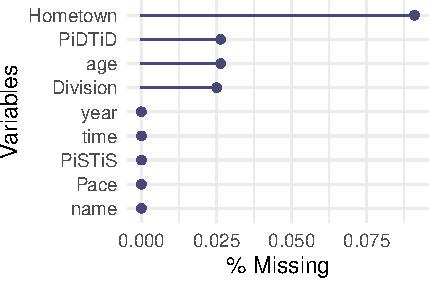
\includegraphics{case_study02_SO02_files/figure-latex/unnamed-chunk-6-1} 

}

\caption{Missing Values}\label{fig:unnamed-chunk-6}
\end{figure}

\hypertarget{impute-or-drop-missing-values}{%
\subsection{Impute or Drop Missing
values}\label{impute-or-drop-missing-values}}

In R VIM package can be use to determine MCAR, MAR and MNAR conditions
on missing data.{[}3{]}{[}4{]}

\begin{figure}[H]

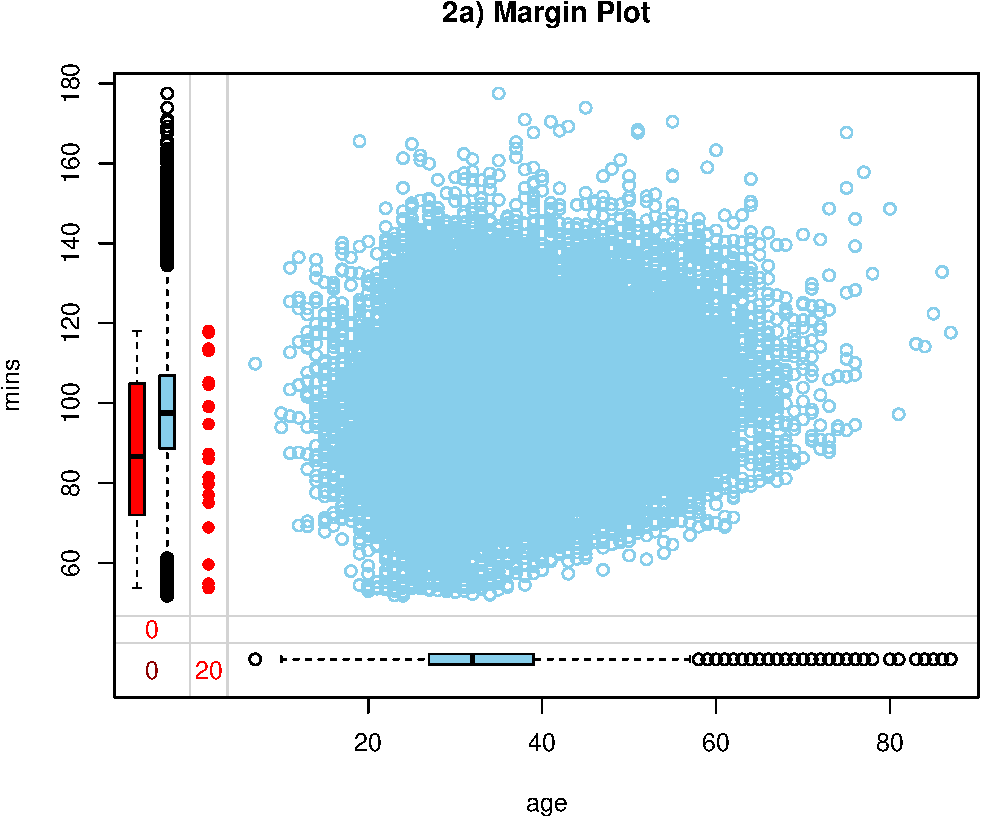
\includegraphics[width=.49\linewidth,]{case_study02_SO02_files/figure-latex/unnamed-chunk-7-1} 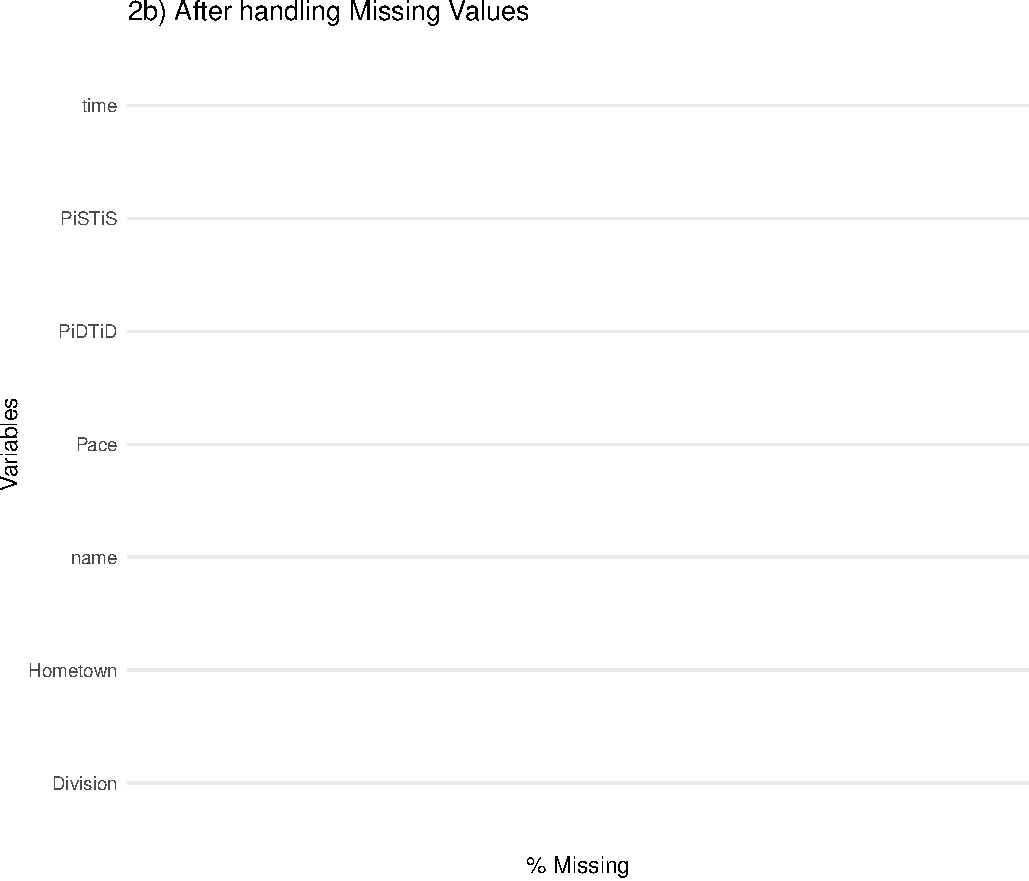
\includegraphics[width=.49\linewidth,]{case_study02_SO02_files/figure-latex/unnamed-chunk-7-2} \hfill{}

\caption{Missing Values Actions}\label{fig:unnamed-chunk-7}
\end{figure}

Interpretation of the marginplot goes as follows:

\begin{itemize}
\tightlist
\item
  From the left vertical boxplots, blue is distribution of minutes when
  age is present
\item
  Red boxplot distribution of minutes when age is not present.
\item
  Age values are missing at 0.02\% also from red and blue boxplot show
  these distributions are overlapping
\item
  Therefore missing values doesn't seem to violate MCAR assumptions.
\item
  Values are Missing Completely at random and hence removing these
  values will not create any bias.
\item
  Imputation is not required therefore 19 observations have been
  removed.
\item
  Missing Hometown values are replaced by ``UNKNOWN'' hometown.
\item
  After removing rows with NA in age, only one value is NA in column
  PiDTiD, upon observation it was found that this player shares rank
  under women category and they both belong to same Division and
  apparently shares same rank in the divison as well. Therefore Rank in
  her division has hard-coded to ``961/1257'' where 961 is her rank and
  1257 is total player in her division.
\item
  Plot 2b) shows there is nothing missing in the data after handling all
  missing values.
\end{itemize}

\hypertarget{preparing-final-dataset}{%
\subsection{Preparing final dataset}\label{preparing-final-dataset}}

Final dataset now contains following fields. Few variables are derived
from the original and changed their datatypes as follows.

e.g.~PiDTiD is character string made up of Rank in Division and Total
Runners in Division.

e.g.~9/100 indicates runner's rank is 9 in his division and there are
total 100 runners in his division. These values are split into two
columns in the final dataset.

Table shows which are orignal fields and which are derived and from
which it is derived.

\begin{longtable}[]{@{}llll@{}}
\caption{Final structure of dataframe}\tabularnewline
\toprule
Field Name & Original/Derived & Data Type & Field
Description\tabularnewline
\midrule
\endfirsthead
\toprule
Field Name & Original/Derived & Data Type & Field
Description\tabularnewline
\midrule
\endhead
Year & Original & Integer & Year of participation\tabularnewline
Name & Original & String & Last Name and First Name of the
Runner\tabularnewline
Age & Original & Integer & Age\tabularnewline
mins & Derived from time & Float & Total Minutes\tabularnewline
PaceMins & Derived from Pace & Float & Miles per hour\tabularnewline
rankWomens & Derived from PiSTiS & Integer & Rank in woman's
category\tabularnewline
TotalWomens & Derived from PiSTiS & Integer & Total women
particiapants\tabularnewline
Division & Original & String & Division\tabularnewline
rankDivision & Derived from PiDTiD & Integer & Rank in Runner's
Division\tabularnewline
TotalDivisions & Derived from PiDTiD & Integer & Total Participants in
Division\tabularnewline
HomeTown & Original & String & Runner's Home Town\tabularnewline
country & Derived from Hometown & String & Runner's Home
Country\tabularnewline
\bottomrule
\end{longtable}

\textbf{Structure of dataframe}

\begin{verbatim}
'data.frame':   75846 obs. of  12 variables:
 $ year          : int  1999 1999 1999 1999 1999 1999 1999 1999 ...
 $ name          : chr  "Jane Omoro (W)" "Jane Ngotho (W)" "Eunice Sagero (W)" ...
 $ age           : int  26 29 20 29 24 38 27 30 ...
 $ mins          : num  53.6 53.6 53.9 54.1 ...
 $ PaceMins      : num  5.37 5.37 5.4 5.42 ...
 $ rankWomens    : int  1 2 4 5 6 7 9 10 ...
 $ TotalWomens   : int  2358 2358 2358 2358 2358 2358 2358 2358 ...
 $ Division      : chr  "W2529" "W2529" "W2024" ...
 $ rankDivision  : num  1 2 1 3 2 1 4 1 ...
 $ TotalDivisions: chr  "559" "559" "196" ...
 $ Hometown      : chr  "Kenya" "Kenya" "Kenya" ...
 $ country       : chr  "Kenya" "Kenya" "Kenya" ...
\end{verbatim}

\hypertarget{summary-of-the-data}{%
\subsection{Summary of the data}\label{summary-of-the-data}}

\begin{verbatim}

+--------------+------------------+---------------+----------------+
|     year     |       name       |      age      |      mins      |
+==============+==================+===============+================+
| Min.  :1999  |   Length:75846   | Min.  : 7.00  | Min.  : 51.73  |
+--------------+------------------+---------------+----------------+
| 1st Qu.:2005 | Class :character | 1st Qu.:27.00 | 1st Qu.: 88.65 |
+--------------+------------------+---------------+----------------+
| Median :2008 | Mode :character  | Median :32.00 | Median : 97.48 |
+--------------+------------------+---------------+----------------+
|  Mean :2007  |        NA        |  Mean :33.85  |  Mean : 98.22  |
+--------------+------------------+---------------+----------------+
| 3rd Qu.:2010 |        NA        | 3rd Qu.:39.00 | 3rd Qu.:106.97 |
+--------------+------------------+---------------+----------------+
| Max.  :2012  |        NA        | Max.  :87.00  | Max.  :177.52  |
+--------------+------------------+---------------+----------------+

Table: Table continues below

 

+----------------+--------------+--------------+------------------+
|    PaceMins    |  rankWomens  | TotalWomens  |     Division     |
+================+==============+==============+==================+
| Min.  : 5.167  |  Min.  : 1   | Min.  :2166  |   Length:75846   |
+----------------+--------------+--------------+------------------+
| 1st Qu.: 8.867 | 1st Qu.:1357 | 1st Qu.:4333 | Class :character |
+----------------+--------------+--------------+------------------+
| Median : 9.750 | Median :2786 | Median :6395 | Mode :character  |
+----------------+--------------+--------------+------------------+
|  Mean : 9.823  |  Mean :3306  |  Mean :6610  |        NA        |
+----------------+--------------+--------------+------------------+
| 3rd Qu.:10.700 | 3rd Qu.:4906 | 3rd Qu.:8853 |        NA        |
+----------------+--------------+--------------+------------------+
| Max.  :17.750  | Max.  :9729  | Max.  :9729  |        NA        |
+----------------+--------------+--------------+------------------+

Table: Table continues below

 

+----------------+------------------+------------------+------------------+
|  rankDivision  |  TotalDivisions  |     Hometown     |     country      |
+================+==================+==================+==================+
|  Min.  : 1.0   |   Length:75846   |   Length:75846   |   Length:75846   |
+----------------+------------------+------------------+------------------+
| 1st Qu.: 165.0 | Class :character | Class :character | Class :character |
+----------------+------------------+------------------+------------------+
| Median : 404.0 | Mode :character  | Mode :character  | Mode :character  |
+----------------+------------------+------------------+------------------+
|  Mean : 595.6  |        NA        |        NA        |        NA        |
+----------------+------------------+------------------+------------------+
| 3rd Qu.: 816.0 |        NA        |        NA        |        NA        |
+----------------+------------------+------------------+------------------+
| Max.  :5302.0  |        NA        |        NA        |        NA        |
+----------------+------------------+------------------+------------------+
\end{verbatim}

\newpage

\hypertarget{exploratory-data-analysis}{%
\subsection{Exploratory Data Analysis}\label{exploratory-data-analysis}}

\hypertarget{age-distributions-participation-over-the-years}{%
\subsubsection{Age Distributions participation over the
years}\label{age-distributions-participation-over-the-years}}

\begin{figure}[H]

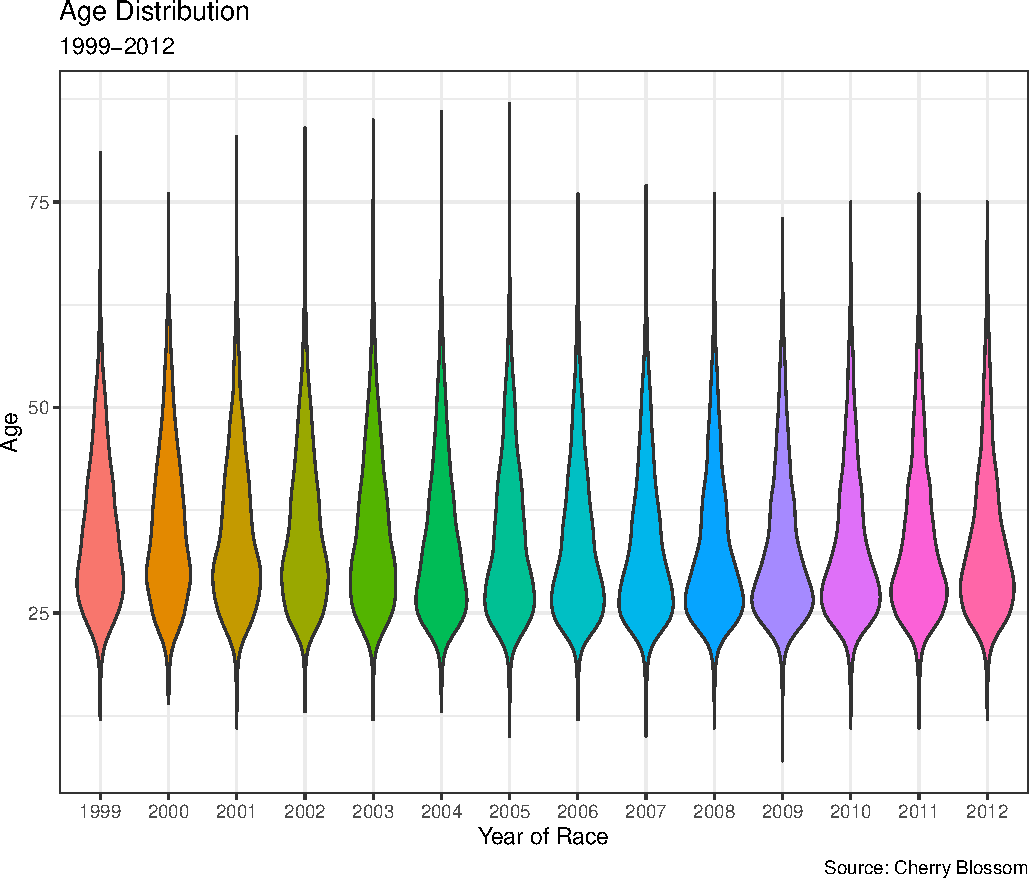
\includegraphics[width=.49\linewidth,]{case_study02_SO02_files/figure-latex/unnamed-chunk-12-1} \hfill{}

\caption{Year wise Distribution}\label{fig:unnamed-chunk-12}
\end{figure}

The Age Distribution chart from 1999-2012 shows over the course of time
the average age has remained relatively constant. 25-30 year olds make
up majority of the race population and that's consistent throughout the
years the races were held.

\begin{figure}[H]

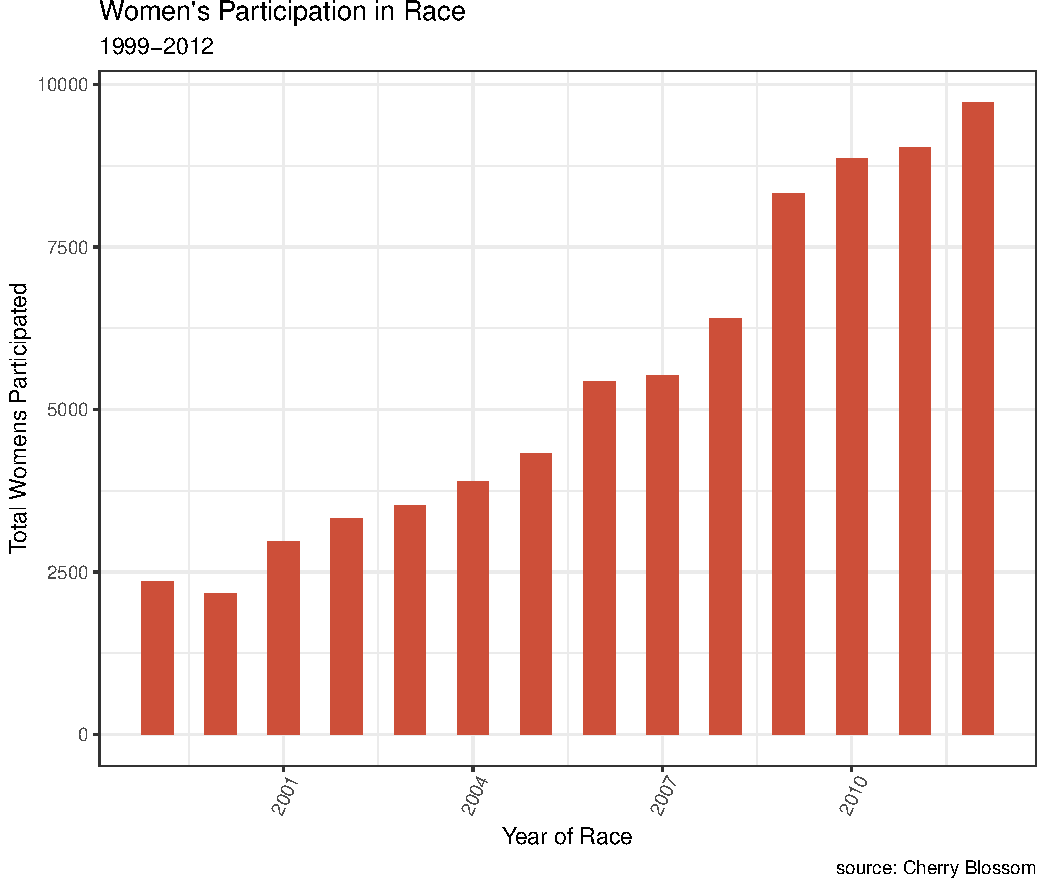
\includegraphics[width=.49\linewidth,]{case_study02_SO02_files/figure-latex/unnamed-chunk-13-1} \hfill{}

\caption{Year wise Distribution}\label{fig:unnamed-chunk-13}
\end{figure}

Looking into the participation, its going up over time, in 1999 they had
around 2,500 participants and it went up to 100,000 in 2012 almost a 4x
increase in participation.

\begin{Shaded}
\begin{Highlighting}[]
\CommentTok{\#cb\_final\_ds$age \textless{}{-} as.numeric(cb\_final\_ds$age)}
\CommentTok{\#cb\_final\_ds$PaceMins \textless{}{-} as.character(cb\_final\_ds$PaceMins)}

\NormalTok{yr\_cnt }\OtherTok{\textless{}{-}} \FunctionTok{count}\NormalTok{(cb\_final\_ds,year)}

\NormalTok{tformat }\OtherTok{\textless{}{-}} \FunctionTok{hms}\NormalTok{(cb\_final\_ds}\SpecialCharTok{$}\NormalTok{time)}
\CommentTok{\#cb\_final\_ds$tmins \textless{}{-} hour(tformat)*60 + minute(tformat)  + second(tformat)/60}

\NormalTok{cb\_final\_ds}\SpecialCharTok{$}\NormalTok{ageRange }\OtherTok{=} \FunctionTok{cut}\NormalTok{(cb\_final\_ds}\SpecialCharTok{$}\NormalTok{age,}\AttributeTok{breaks =} \FunctionTok{c}\NormalTok{(}\DecValTok{0}\NormalTok{,}\DecValTok{15}\NormalTok{,}\DecValTok{25}\NormalTok{,}\DecValTok{45}\NormalTok{,}\DecValTok{65}\NormalTok{,}\DecValTok{90}\NormalTok{))}

\NormalTok{age\_yr\_cnt }\OtherTok{\textless{}{-}}\NormalTok{ (cb\_final\_ds }\SpecialCharTok{\%\textgreater{}\%} \FunctionTok{group\_by}\NormalTok{(ageRange) }\SpecialCharTok{\%\textgreater{}\%} \FunctionTok{count}\NormalTok{(year) }\SpecialCharTok{\%\textgreater{}\%} \FunctionTok{mutate}\NormalTok{(}\AttributeTok{Nor =}\NormalTok{ n}\SpecialCharTok{/}\NormalTok{n[}\DecValTok{1}\NormalTok{])) }\SpecialCharTok{\%\textgreater{}\%} \FunctionTok{mutate}\NormalTok{(}\AttributeTok{n\_diff =}\NormalTok{ n }\SpecialCharTok{{-}} \FunctionTok{lag}\NormalTok{(n))}

\NormalTok{cb\_final\_ds}\SpecialCharTok{$}\NormalTok{ageRange\_gran }\OtherTok{=} \FunctionTok{cut}\NormalTok{(cb\_final\_ds}\SpecialCharTok{$}\NormalTok{age,}\AttributeTok{breaks =} \FunctionTok{c}\NormalTok{(}\FunctionTok{seq}\NormalTok{(}\DecValTok{0}\NormalTok{,}\DecValTok{90}\NormalTok{,}\DecValTok{10}\NormalTok{)))}

\NormalTok{age\_gran\_yr\_cnt }\OtherTok{\textless{}{-}}\NormalTok{ (cb\_final\_ds }\SpecialCharTok{\%\textgreater{}\%} \FunctionTok{group\_by}\NormalTok{(ageRange\_gran) }\SpecialCharTok{\%\textgreater{}\%} \FunctionTok{count}\NormalTok{(year) }\SpecialCharTok{\%\textgreater{}\%} \FunctionTok{mutate}\NormalTok{(}\AttributeTok{Nor =}\NormalTok{ n}\SpecialCharTok{/}\NormalTok{n[}\DecValTok{1}\NormalTok{])) }\SpecialCharTok{\%\textgreater{}\%} \FunctionTok{mutate}\NormalTok{(}\AttributeTok{n\_diff =}\NormalTok{ n }\SpecialCharTok{{-}} \FunctionTok{lag}\NormalTok{(n))}

\CommentTok{\#age\_yr\_time \textless{}{-} (cb\_final\_ds \%\textgreater{}\% group\_by(ageRange\_gran,year) \%\textgreater{}\% mutate(t\_median = median(tmins)) \%\textgreater{}\% mutate(t\_min = min(tmins)))}
\end{Highlighting}
\end{Shaded}

\begin{Shaded}
\begin{Highlighting}[]
\FunctionTok{ggplot}\NormalTok{(age\_gran\_yr\_cnt, }\FunctionTok{aes}\NormalTok{(}\AttributeTok{x =}\NormalTok{ year, }\AttributeTok{y =}\NormalTok{ n))}\SpecialCharTok{+}
  \FunctionTok{geom\_line}\NormalTok{(}\FunctionTok{aes}\NormalTok{(}\AttributeTok{color =}\NormalTok{ ageRange\_gran))}\SpecialCharTok{+}
  \FunctionTok{labs}\NormalTok{(}\AttributeTok{title=}\StringTok{"Women Participation }\SpecialCharTok{\textbackslash{}n}\StringTok{ by Age Group"}\NormalTok{,}\AttributeTok{x=}\StringTok{"Year of Race"}\NormalTok{, }\AttributeTok{y =} \StringTok{"Womens Participants"}\NormalTok{)}\SpecialCharTok{+}
  \FunctionTok{theme\_minimal}\NormalTok{()}\SpecialCharTok{+}
  \FunctionTok{theme}\NormalTok{(}\AttributeTok{plot.title =} \FunctionTok{element\_text}\NormalTok{(}\AttributeTok{hjust =} \FloatTok{0.5}\NormalTok{))}
\end{Highlighting}
\end{Shaded}

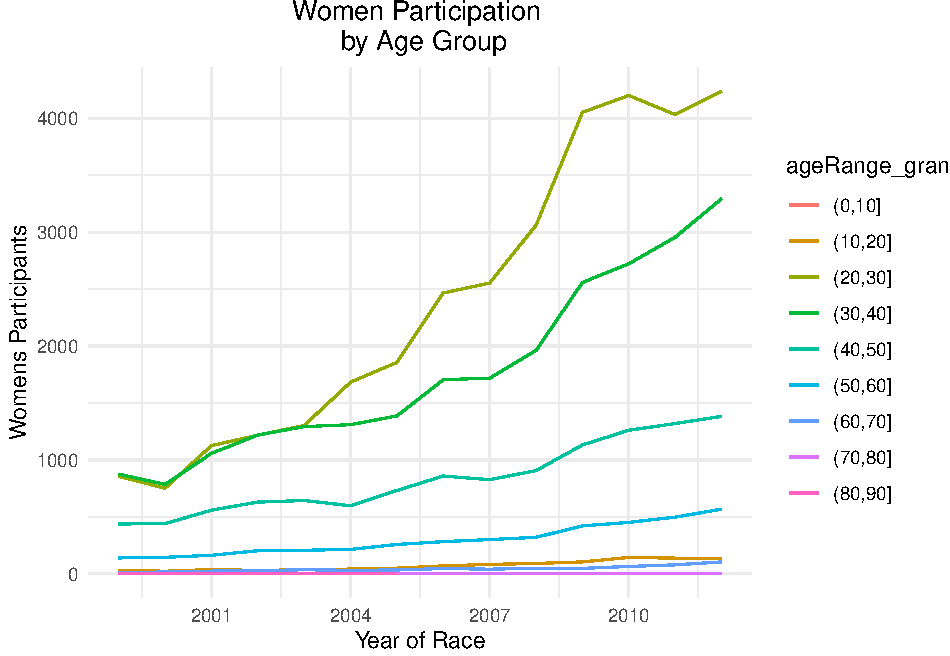
\includegraphics{case_study02_SO02_files/figure-latex/analysis9-1}
Participation was up among all women age groups over the years. There's
a significant increase in women aged 20-30(4x) and also 30-40(3.5x)
participation from 1999 to 2012.

\begin{Shaded}
\begin{Highlighting}[]
\FunctionTok{ggplot}\NormalTok{(}\FunctionTok{na.omit}\NormalTok{(cb\_final\_ds), }\FunctionTok{aes}\NormalTok{(}\AttributeTok{x =}\NormalTok{ ageRange\_gran, }\AttributeTok{y =}\NormalTok{ mins))}\SpecialCharTok{+}
  \FunctionTok{geom\_boxplot}\NormalTok{()}\SpecialCharTok{+}
  \FunctionTok{labs}\NormalTok{(}\AttributeTok{title=}\StringTok{"Runtime Distribution by Age Group"}\NormalTok{,}\AttributeTok{x=}\StringTok{"Age Group"}\NormalTok{, }\AttributeTok{y =} \StringTok{"Runtime, minutes"}\NormalTok{)}\SpecialCharTok{+}
  \FunctionTok{theme\_minimal}\NormalTok{()}\SpecialCharTok{+}
  \FunctionTok{theme}\NormalTok{(}\AttributeTok{plot.title =} \FunctionTok{element\_text}\NormalTok{(}\AttributeTok{hjust =} \FloatTok{0.5}\NormalTok{))}
\end{Highlighting}
\end{Shaded}

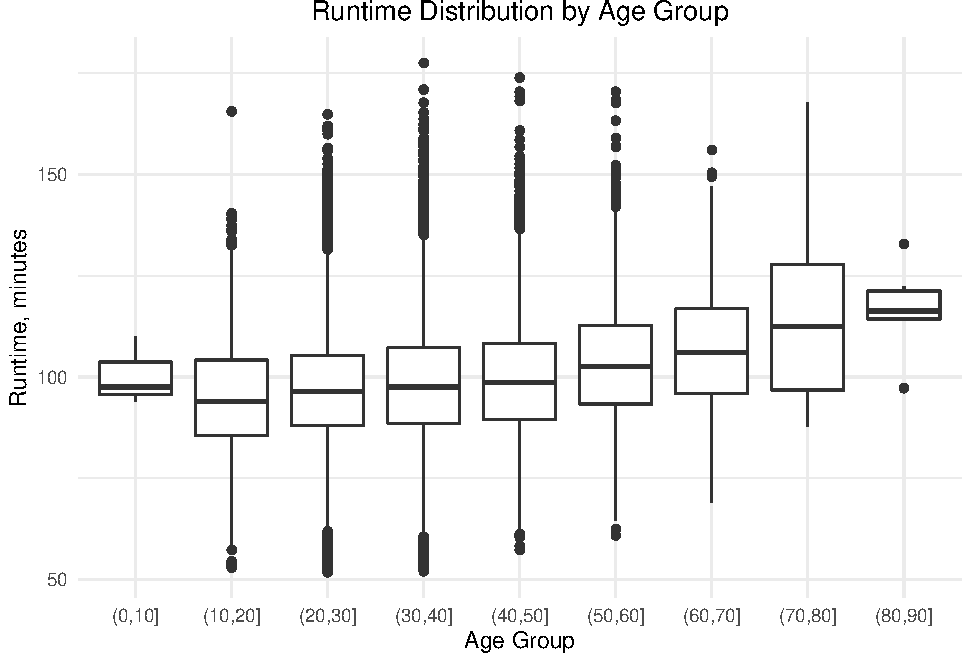
\includegraphics{case_study02_SO02_files/figure-latex/analysis16-1}

\begin{Shaded}
\begin{Highlighting}[]
\FunctionTok{ggplot}\NormalTok{(cb\_final\_ds, }\FunctionTok{aes}\NormalTok{(}\AttributeTok{x =} \FunctionTok{factor}\NormalTok{(year), }\AttributeTok{y =}\NormalTok{ mins))}\SpecialCharTok{+}
  \FunctionTok{geom\_boxplot}\NormalTok{()}\SpecialCharTok{+}
  \FunctionTok{labs}\NormalTok{(}\AttributeTok{title=}\StringTok{"Runtime Distribution by Year"}\NormalTok{,}\AttributeTok{x=}\StringTok{"Year"}\NormalTok{, }\AttributeTok{y =} \StringTok{"Runtime, minutes"}\NormalTok{)}\SpecialCharTok{+}
  \FunctionTok{theme\_minimal}\NormalTok{()}\SpecialCharTok{+}
  \FunctionTok{theme}\NormalTok{(}\AttributeTok{plot.title =} \FunctionTok{element\_text}\NormalTok{(}\AttributeTok{hjust =} \FloatTok{0.5}\NormalTok{))}
\end{Highlighting}
\end{Shaded}

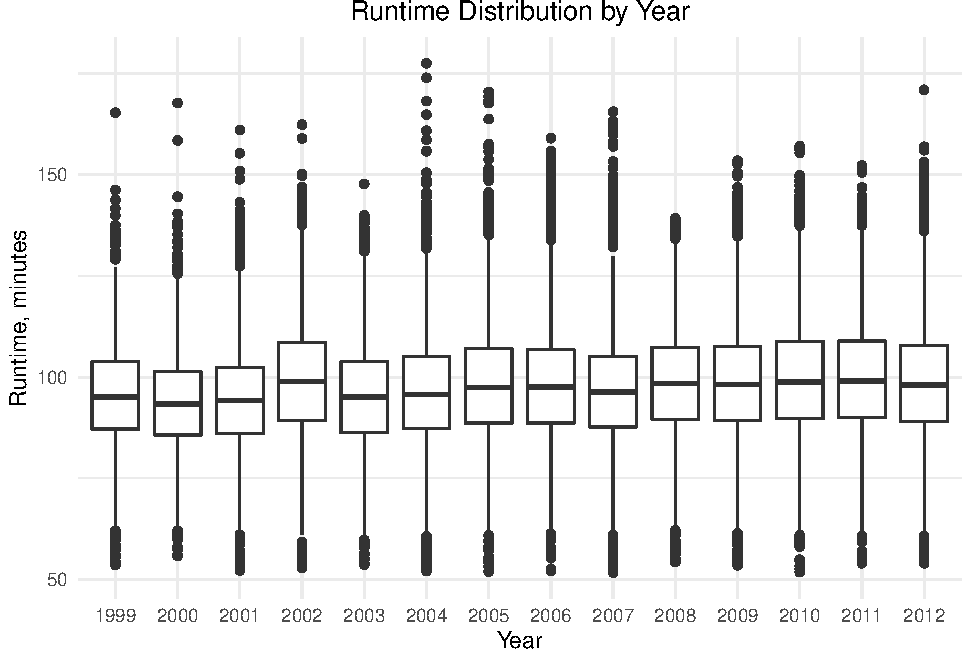
\includegraphics{case_study02_SO02_files/figure-latex/analysis14-1}

\newpage

\hypertarget{business-analysis}{%
\section{Business Analysis}\label{business-analysis}}

\newpage

\hypertarget{conclusion}{%
\section{Conclusion}\label{conclusion}}

\hypertarget{references}{%
\section*{References}\label{references}}
\addcontentsline{toc}{section}{References}

{[}1{]} Deborah Nolan; Duncan Temple Lang. Data Science in R.Chapman and
Hall/CRC, 2015.

{[}2{]}
\href{https://www.bls.gov/opub/ted/2016/sports-and-exercise-among-americans.htm}{Sports
and exercise among Americans : The Economics Daily: U.S. Bureau of Labor
Statistics}

{[}3{]} Templ, Matthias \& Alfons, Andreas \& Filzmoser, Peter. (2012).
Exploring incomplete data using visualization techniques. Advances in
Data Analysis and Classification. 6. 29-47. 10.1007/s11634-011-0102-y.

{[}4{]}
\href{https://boostedml.com/2020/05/visualizing-missing-data-in-r-the-basics-with-vim.html\#The_Margin_Plot_Checking_Missing_Completely_at_Random_MCAR}{Example
of interpretation of VIM::marginplot}

\end{document}
